\documentclass[pdftex,a4paper,12pt]{article}
\usepackage[T2A]{fontenc}
\usepackage[russian]{babel}
%\usepackage{ucs}
\usepackage[utf8]{inputenc}
\usepackage{graphicx}
\usepackage[font=small,labelfont=bf]{caption}
\usepackage[unicode=true]{hyperref}
\hypersetup{
		pdftitle={Богданов Д.А., “Численное исследование течения в фильтре-циклоне”, 2012},
    colorlinks,
    citecolor=black,
    filecolor=black,
    linkcolor=black,
    urlcolor=black
}
\title{Численное исследование течения в фильтре-циклоне}
\author{Дмитрий Богданов}
\date{}
\begin{document}
\renewcommand\normalsize{\fontsize{12pt}{14pt}\selectfont}
\begin{titlepage}
	\begin{center}
		\small{МИНИСТЕРСТВО ОБРАЗОВАНИЯ И НАУКИ \\ РОССИЙСКОЙ ФЕДЕРАЦИИ \\
Санкт-Петербургский государственный политехнический университет \\
Физико-механический факультет \\
Кафедра гидроаэродинамики}\\
		\vspace{0.18\textheight}
	\end{center}
	\begin{center}
		\vspace{0.1\textheight}
		\large{Численное исследование течения в фильтре-циклоне}\\
		\vspace{0.01\textheight}
		\normalsize
		\textsc{Автореферат диссертации на соискание ученой степени магистра по направлению 010600 – Прикладные математика и физика}
		\vspace{0.25\textheight}
	\end{center}
	\begin{minipage}{0.48\textwidth}
		\begin{flushleft}
			Выполнил студент гр. 6054/11\\
			Руководитель, к.ф.-м.н., с.н.с.\\
		\end{flushleft}
	\end{minipage}
	\begin{minipage}{0.5\textwidth}
		\begin{flushright}
			Богданов Д.А. \\
			Поняев С.А. \\
		\end{flushright}
	\end{minipage}
	\vspace{0.1\textheight}
	\begin{center}
		Санкт-Петербург \\
		\the\year
	\end{center}
\end{titlepage}
\newpage
\renewcommand\normalsize{\fontsize{14pt}{24pt}\selectfont}
\tableofcontents
\newpage
\section{Введение}
	\subsection{Актуальность проблемы}
		\hspace{2em} 	Задача очищения атмосферного воздуха от загрязняющих выбросов промышленных предприятий достаточно актуальна. Выбросы от стационарных источников вредных веществ в атмосферу городов и населенных пунктов, расположенных на территории северо-западного федерального округа,  по данным Росстата за 2007 год,  составили 2319000 тонн, в том числе твёрдых -- 289400 тонн \cite{emissionInfoRussian}.
		\begin{figure}[ht]
			\vspace{-1em}
			\begin{minipage}[b]{0.46\linewidth}
				В некоторых отраслях промышленности доля выбросов пыли в атмосферу достигает 15\% от общего числа получаемого продукта. Так, при изготовлении одной тонны цемента в воздух выбрасывается $\approx 160$ кг цементной пыли \cite{emissionInfoEurope}.
				Динамика изменения объёма выбросов твёрдых вредных веществ в атмосферу \textit{(рис. \ref{figure:atmosphereDynamic})} имеет тенденцию к росту, что говорит о том, что решение проблемы инженерной защиты воздуха от вредных веществ останется актуальной и в ближайшем будущем. 
			\end{minipage}
			\hspace{0.01\linewidth}
			\begin{minipage}[b]{0.48\linewidth}
				\centering
				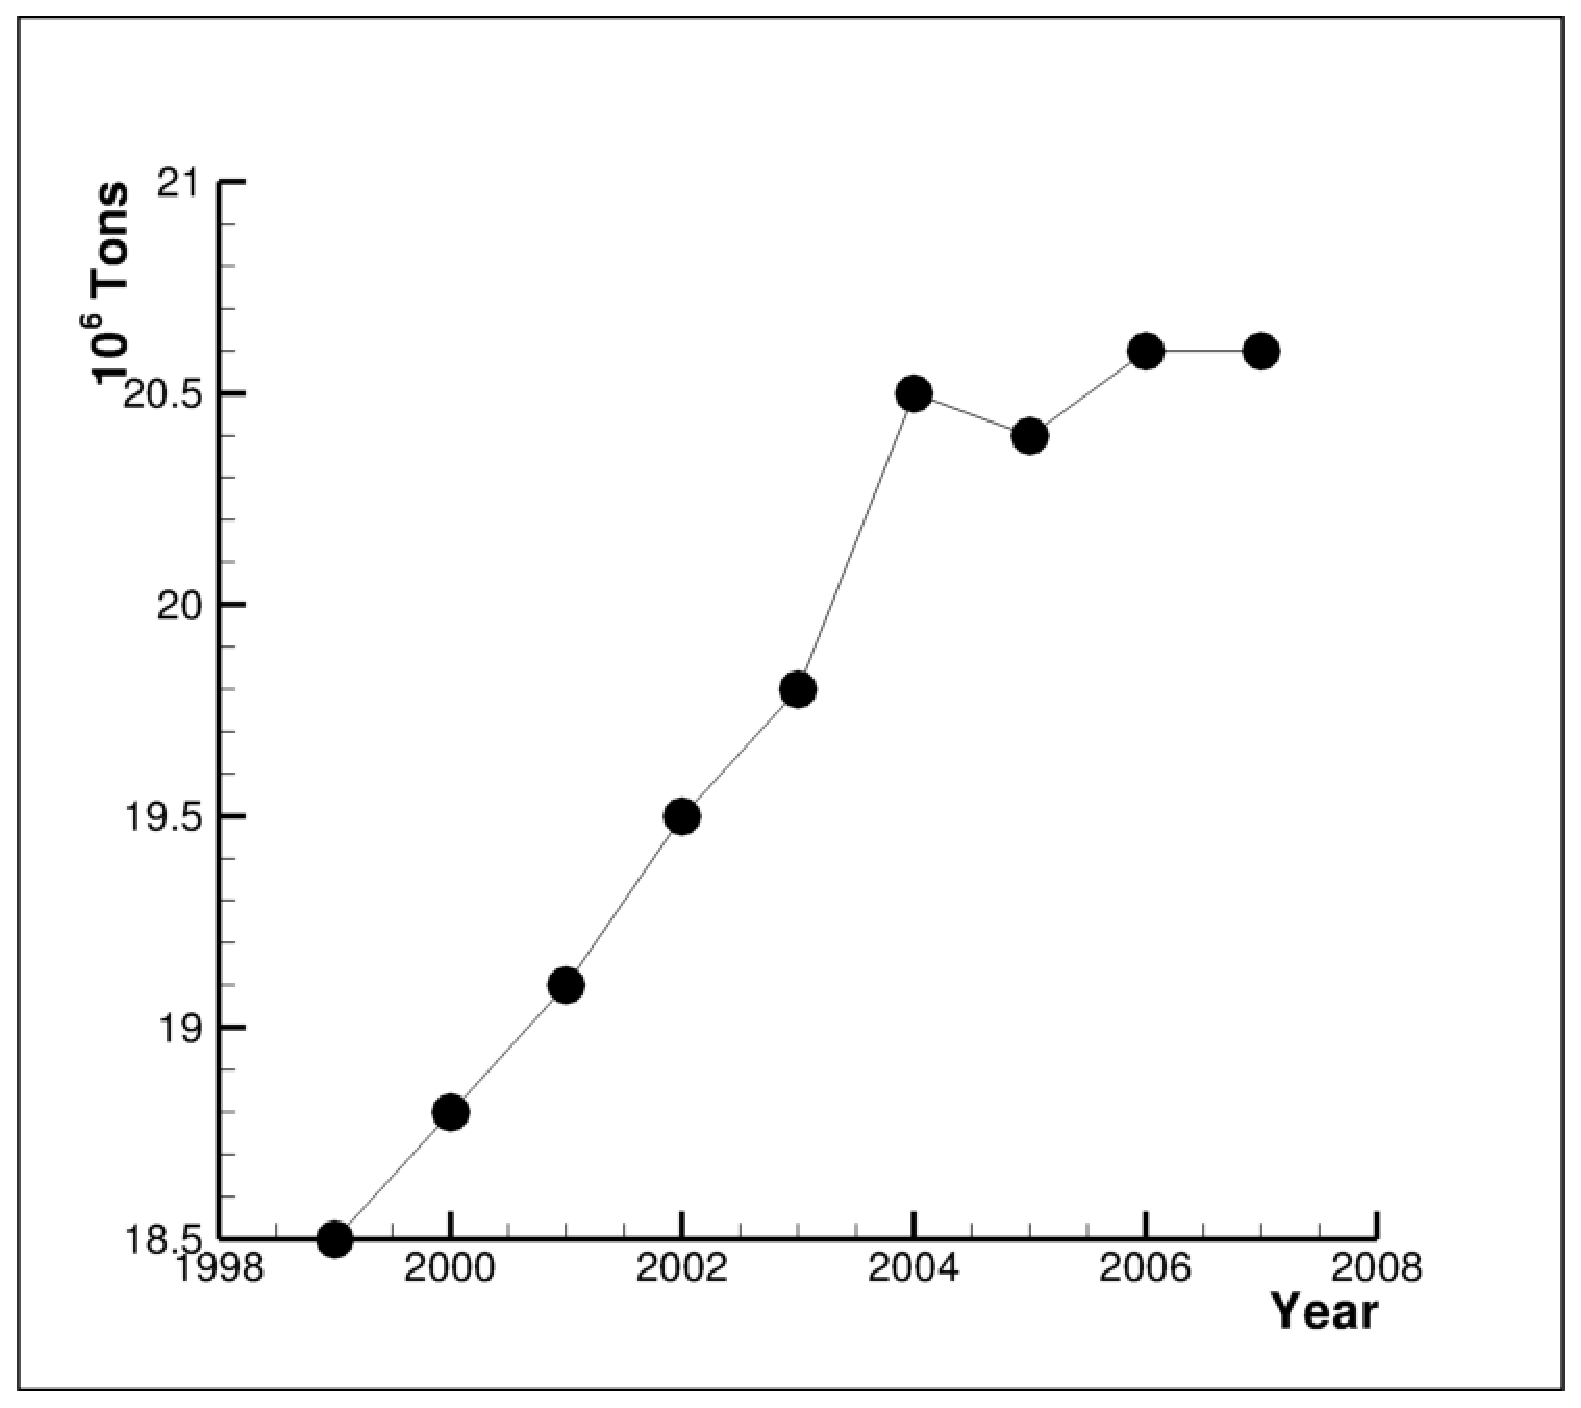
\includegraphics[scale=0.24]{atmosphereDynamic}
				\caption{Динамика выбросов твёрдых вредных веществ в атмосферу \cite{emissionInfoRussian}}
				\label{figure:atmosphereDynamic}
			\end{minipage}
		\end{figure}
		\vspace{-1em}
	
		Для очищения воздуха от твёрдых примесей широкое распространение получили фильтры типа циклон. Циклон представляет собой инерционный пылеуловитель, в котором выделение частиц из воздушной среды происходит, в основном, под действием центробежной силы, возникающей при вращении воздушного потока в корпусе аппарата.
	
		Запылённый воздух входит в циклон через тангенциальный патрубок и, приобретая вращательное движение, опускается винтообразно вниз вдоль внутренних стенок цилиндра и конуса. Небольшая часть этого потока, в котором сконцентрированы пылевые частицы, движется в непосредственной близости от стенок циклона и поступает через пылеотводящее отверстие в пылесборный бункер, где происходит осаждение и накопление пылевых частиц.
	
		В центральной зоне циклона воздушный поток, освобождённый от пыли, поднимается винтообразно вверх и удаляется через выхлопную трубу наружу.
	
		Вследствие вращательного движения воздушного потока в центральной зоне циклона (в конусе, выхлопной трубе и пылесборном бункере) наблюдается пониженное давление.\cite{instructions}
	
		В силу высокой степени закрученности потока, необходимо введение поправок в модели турбулентности для учёта кривизны линий тока. Кроме того, учитывая высокую концентрацию частиц в потоке, в инженерных расчётах необходимо учитывать не только влияние потока на частицы, но также и обратное влияние частиц на поток.
	%Актуальность проблемы
	\subsection{Цели работы}
		\begin{enumerate}
			\item Реализация $k-\omega-SST$ модели турбулентности с поправкой на кривизну линий тока при помощи открытой интегрируемой платформы для численного моделирования задач механики сплошных сред OpenFOAM.
			\item Реализация с использованием OpenFOAM солвера, имеющего в основе модель идеального газа и учитывающего при этом обратное влияние частиц на поток.
			\item Численное моделирование циклона с учётом обратного влияния частиц на поток и поправки на кривизну линий тока к генерации турбулентности.
		\end{enumerate}
	%Цели работы
\newpage
%Введение

\section{Обзор существующих исследований}
	\subsection{Экспериментальные исследования}
		\hspace{2em}Существует большое количество работ по экспериментальному исследованию течения с криволинейными линиями тока. Среди них стоит выделить достаточно подробный эксперимент, приведённый в статье Monson et al. \cite{Monson}. Авторы статьи проводят численное и экспериментальное исследование турбулентного течения воздуха в U-образном канале.
	
		Экспериментальному моделированию циклонов также уделено немало внимания. Среди статей, приводящих экспериментальные данные по турбулентному течению в циклонах, нужно отметить детальное исследование течения в циклоне модели Stairmand, описанное в статье J. Dirgo, D. Leith \cite{DirgoLeith}. В этой статье приведены данные для профилей скорости в нескольких сечениях фильтра для большого диапазона рабочих параметров. К сожалению!!!!!!!!!!!!!!!!!!!!!!!!!!!1
	\subsection{Теоретические исследования}
		\hspace{2em}Среди теоретических исследований течения в циклонах особо выделим статью 
	\subsection{Численные исследования}
		\hspace{2em}Численному моделированию течения в циклонах посвящено очень много инженерных исследований.
	%Численные исследования
\newpage
%Обзор существующих моделей
\section{Численное моделирование}
	\subsection{Уравнения движения}
		\subsubsection{Уравнение баланса массы}
			\begin{equation}
				\frac{\partial \rho}{\partial t} + \frac{\partial}{\partial x_i}(\rho u_i) = 0
			\end{equation}
		\subsubsection{Уравнение баланса импульса}
			\begin{equation}
				\frac{\partial \rho u_i}{\partial t} + \frac{\partial}{\partial x_j}(\rho u_iu_j) = - \frac{\partial p}{\partial x_i} + \frac{\partial {\tau_{ij}}_{eff}}{\partial x_j},
			\end{equation}
			где ${\tau_{ij}}_{eff}$ - тензор вязких напряжений, выражаемый по формуле
			\begin{equation}
				{\tau_{ij}}_{eff} = \mu_{eff}\left( \frac{\partial u_i}{\partial x_j} + \frac{\partial u_j}{\partial x_i} \right) - \frac{2}{3}\mu_{eff}\frac{\partial u_i}{\partial x_j} \delta_{ij} \quad \mu_{eff} = \mu + \mu_{t}
			\end{equation}
		\subsubsection{Уравнение баланса энтальпии}
		\subsubsection{Уравнение состояния}
			\hspace{2em}При расчётах течений сжимаемой жидкости используется модель идеального газа:
			\begin{equation}
				\frac{p}{\rho} = \frac{R}{m}T, \quad m = 28.966 \frac{kg}{mole}
			\end{equation}
			\subsubsection{Зависимость вязкости от температуры}
				\hspace{2em}Зависимость вязкости от температуры выражается формулой Саттерленда для сильно неизотермических течений.
				\begin{equation}
					\mu = \mu_0 \frac{T_0 + C}{T + C_0} \frac{T^{\frac{3}{2}}}{T}, \quad \mu_0 = 1.73 \cdot 10^{-5} kg \cdot m/s, \quad T_0 = 273K, \quad C=110 K
				\end{equation}
				Для течений, температура в которых меняется слабо, вязкость полагается постоянной.
	%Основные уравнения
	\newpage
	\subsection{Модель турбулентности}
		\hspace{2em}
		Основой правильного численного моделирования течений сжимаемых сред является надёжная и стабильная модель турбулентности. Опыт использования моделей турбулентности показывает, что более высокотехнологичные модели имеют не слишком большое преимущество над хорошо откалиброванными моделями турбулентной вязкости.
		
		Модель турбулентной вязкости, тем не менее, должна удовлетворять ряду требований для того, чтобы правильно предсказать основные характеристики пограничного слоя. Основным требованием является то, что модель должна ограничивать завышенную генерацию турбулентности в застойных зонах, которая наблюдается в стандартных моделях с двумя уравнениями. В частности, для предсказания теплообмена эти нефизично высокие уровни турбулентности оказывают сильное влияние на скорость передачи тепла в пограничном слое. Для преодоления этого недостатка используются различные модификации стандартных формулировок моделей турбулентности, как то ограничитель генерации, предложенный Menter (1994) или $k-\varepsilon$ модель Kato-Launder (1993).
		
		Существенной особенностью пограничного слоя является его отрыв от поверхности при неблагоприятном градиенте давления. Отрыв имеет сильное влияние на характеристики турбулентности, а следовательно, и на теплообмен. SST-модель показала отличные	 возможности предсказания точек отрыва пограничного слоя и наиболее часто используется для анализа течений с теплообменом. Идея SST-модели состоит в сочетании лучших элементов $k-\omega$ и $k-\varepsilon$ моделей при помощи перекрёстной функций $F_1$, которая равна единице на твёрдой поверхности и нулю вне пограничного слоя. Таким образом, автоматически используется $k-\omega$ модель Wilcox  в пристеночной области и $k-\varepsilon$ для остальной части потока. Такой подход позволяет использовать эффективную модель Wilcox в пристенных областях, не имея при этом потенциальных ошибок, связанных с чувствительностю модели Wilcox в свободных сдвиговых потоках. В SST-модели также используется несколько отличное от традиционного выражение для определения турбулентной вязкости, которое может быть интерпретировано, как введение в формулу для $\mu_t$ коэффициента $c_{\mu}$. Эта модификация необходима для того, чтобы правильно предсказать точку отрыва пограничного слоя под действием встречного градиента давления. \cite{Menter}
		Формулировка SST-модели турбулентности следующая:
		\newpage
		\subsubsection{Уравнение баланса кинетической энергии турбулентности}
				\begin{equation}
				\frac{\partial \rho k}{\partial t} + \frac{\partial \rho U_j k}{\partial x_j} = \tilde{P}_k f_{rot} - \beta^* \rho k \omega + \frac{\partial}{\partial x_j}(\Gamma_k \frac{\partial k}{\partial x_j}),
				\end{equation}
				где $f_{rot}$ - поправочный коэффициент Шура-Спалларта к генерации турбулентности, учитывающий криволинейность потока, определяемый в \ref{CC}.
		\subsubsection{Уравнение баланса удельной скорости диссипации}
			\begin{equation}
				\frac{\partial \rho \omega}{\partial t} + \frac{\partial U_j \omega}{\partial x_j} = \frac{\gamma}{\nu_t}P_k - \beta\rho\omega^2 + \frac{\partial}{\partial x_j}(\Gamma_{\omega}\frac{\partial \omega}{\partial x_j}) + (1-F_1)2\rho \sigma_{\omega_2}\frac{1}{\omega}\frac{\partial k}{\partial x_j}\frac{\partial \omega}{\partial x_j},
			\end{equation}
			где
			\small{
			\begin{equation}
				\Gamma_k = \mu + \frac{\mu_t}{\sigma_k}, \Gamma_{\omega} = \mu + \frac{\mu_t}{\sigma_{\omega}}, P_k = \tau_{ij}\frac{\partial U_i}{\partial x_j}, \tilde{P}_k = min(P_k, c_1\varepsilon), \mu_t=\rho\frac{a_1 k}{max(a_1\omega, S \cdot F_2)}
			\end{equation}
			}
			
			Коффициент $\phi$ в модели представляет собой функцию от $F_1$: $\phi = F_1\phi_1 + (1-F_1)\phi_2$, где $\phi_1$ и $\phi_2$ соответственно коеффициенты для $k-\omega$ и $k-\varepsilon$ моделей.
			$$
				\sigma_{k1} = 1.176, \quad \sigma_{\omega 1} = 2.0, \quad \gamma_1 = 0.5532 \quad \beta_1=0.075, \quad \beta^*=0.09, \quad c_1 = 10,
			$$
			$$
				\sigma_{k2} = 1.0, \quad \sigma_{\omega 2} = 1.168, \quad \gamma_2 = 0.4403 \quad \beta_2=0.0828, \quad \beta^*=0.09, \quad \kappa = 0.41
			$$
			\begin{eqnarray}
				F_1 &=& \tanh{(arg_1^4)}, \quad arg_1 = \min\left[\max\left(\frac{\sqrt{k}}{\beta^*\omega y},\frac{500 \nu}{y^2 \omega} \right), \frac{4\rho\sigma_{\omega 2}k}{CD_{k\omega}y^2}\right] \\ \nonumber CD_{k\omega} &=& \max\left( 2\rho\sigma_{\omega_2}\frac{1}{\omega}\frac{\partial k}{\partial x_j}\frac{\partial \omega}{\partial x_j},10^{-10} \right) \\
				F_2 &=& \tanh{(arg_2^2)}, \quad arg_2 = \max\left(2\frac{\sqrt{k}}{\beta^*\omega y},\frac{500 \nu}{y^2\omega}\right) \\
				\nonumber \tau_{ij} &=& \mu_t\left( \frac{\partial U_i}{\partial x_j} + \frac{\partial U_j}{\partial x_i} - \frac{2}{3}\frac{\partial U_k}{\partial U_k}\right) - \frac{2}{3}\rho k \delta_{ij}
			\end{eqnarray}
			\newpage
			\subsubsection{Турбулентный тепловой поток}
			По аналогии с тензором турбулентных напряжений, турбулентный тепловой поток моделируется при помощи турбулентной диффузии:
				\begin{equation}
					\overline{u^{'}_jT^{'}} = - \varepsilon \frac{\partial T}{\partial x_j} = -\frac{\nu_t}{Pr_t}\frac{\partial T}{\partial x_j}, \quad Pr_t = \frac{\nu_t}{\varepsilon_h}
				\end{equation}
				В силу того, что число Прандтля является свойством вещества, турбулентное число Прандтля полагается постоянным исходя из аналогии между турбулентным теплопереносом и массопереносом. Экспериментальные и теоретические исследования показывают, что турбулентное число Прандтля примерно равно $0.9$.
			\subsubsection{Автоматические пристеночные функции}
				В силу того, что пристеночные функции некорректны в случае достаточно подробной сетки, желательно иметь возможность точно разрешать течение в вязком подслое, решая уравнения вплоть до твёрдой поверхности. Идея автоматических пристеночных функций состоит в том, что модель постепенно переходит от формулировки вязкого подслоя к пристеночным функциям в зависимости от подробности расчётной сетки. Уравнение переноса $\omega$ крайне удачный выбор в этом плане, так как оно имеет аналитическое решение как для вязкого подслоя, так и для логарифмического региона. Таким образом, необходимо только определить общую зависимость, основанную на величине $y^{+}$.
				
				Решение для $\omega$ в вязком подслое и логарифмическом регионе:
				\begin{equation}
					\omega_{vis} = \frac{6\nu}{0.075 y^2}, \quad \omega_{log} = \frac{1}{0.3 \kappa}\frac{u_{\tau}}{y}
				\end{equation}
				Это решение может быть переформулировано в терминах $y^{+}$:
				\begin{equation}
						u_{\tau}^{vis} = \frac{U_1}{y^{+}}, \quad u_{\tau}^{log} = \frac{U_1}{\frac{1}{\kappa}\ln(y^{+})+C}, \quad u_{\tau} = {}^4\sqrt{(u_{\tau}^{vis})^4 + (u_{\tau}^{log})^4}
				\end{equation}
				а результирующая функция записана, как
				\begin{equation}
					\omega_1(y^{+})=\sqrt{\omega^2_{vis}(y^{+})+\omega^2_{log}(y^{+})}.
				\end{equation}
				Согласно \cite{Garbarek}, значение $\omega$ на стенке определяется следующим образом:
		\begin{equation}
			\omega_w = 10 \frac{6\nu}{\beta_1 \triangle{y_1}^2}
		\end{equation}
	\newpage
	\subsubsection{Введение поправки на кривизну линий тока}
		\label{CC}
		Наличие членов, явно учитывающих вклад вращения и кривизны линий тока в уравнениях моделей турбулентности цитируется как фундаментальное преимущество моделей Рейнольдсовых напряжений над более простыми моделями турбулентной вязкости \cite{ShurSpallart}. Внесение эффективных изменений в более простые модели может, тем не менее, иметь широкое применение в силу того \cite{CC2}, что для большого класса вычислительных задач модели Рейнольдсовых напряжений пока не доведены до того состояния, в котором они показали бы свою высокую стабильность и точность расчётов \cite{CC3}.
		
		Влияние вращения и кривизны линий тока на турбулентность проявляется наиболее сильно в двух предельных случаях. В тонких сдвиговых течениях с маленькой, по сравнению со скоростью сдвига, скоростью вращения или слабой кривизной линий тока, наблюдается значительное влияние этих эффектов на уровень турбулентных напряжений \cite{Bradshaw}. Другим крайним случаем является однородное сдвиговое течение во вращающейся области, в котором турбулентные пульсации затухают под влиянием сильного вращения \cite{Speziale}. Другой случай сильного вращения это течение в ядре свободного вихря, моделирование которого также показывают плохие результаты при использовании немодифицированных моделей турбулентности \cite{Govindaraju}.
		
		Для учёта влияния кривизны линий тока в данной работе используется поправка на кривизну линий тока, предложенная для модели Spalart-Almaras в \cite{ShurSpallart} и переформулированная применительно к SST модели в \cite{Smirnov}.
		
		В указанной работе рассматривается сдвиговое течение с базовой скоростью, направленной по оси $x$, а все величины меняются, в основном, в направлении $y$. Пусть $U(y)$ - профиль скорости, и пусть $U_y > 0$ так что $\omega_z < 0$. Состредоточимся на проекции тензора Рейнольдсовых напряжений $-\overline{u^{'}v^{'}}$, которая положительна. Вращение с угловой скоростью $\Omega$ вносит вклад $2\Omega(\overline{{u^{'}}^2}-\overline{{v^{'}}^2})$ в эту величину. Если $\overline{{u^{'}}^2} > \overline{{v^{'}}^2}$, величина касательного напряжения возрастает, и наоборот. Таким образом, генерационный член возникает из-за достаточно тонких особенностей тензора Рейнольдсовых напряжений, которые, конечно, не учитываются в моделях турбулентной вязкости.
		
		В случае криволинейности потока, аналогичный член появляется, если уравнения движения записать в криволинейной системе координат, ориентированной по направлению потока, что приводит к появлению "эффективной скорости вращения", равной $U/R$, где $R$ - радиус кривизны линий тока ($R$ принимается положительной в случае вогнутых линий тока). $U/R$ может быть записана, как $\frac{\partial V}{\partial x}$. Нужно заметить, что $\frac{\partial V}{\partial x}$, несмотря на то, что это частная производная от скорости, не является Галилеевым инвариантом так как это частная производная по оси, сонаправленной с вектором скорости.
		
		Неравнозначность $\overline{{u^{'}}^2} > \overline{{v^{'}}^2}$ в тонком сдвиговом течении эквивалетна тому, что главные оси тензора Рейнольдсовых напряжений не сонаправлены с главными осями сдвиговых деформаций (которые повёрнуты на $45^o$ по отношению к осям $(x, y)$), а повёрнуты против часовой стрелки. Таким образом, оси тензора напряжений опережают, или отстают от осей тензора скоростей деформации по отношению к осям системы координат или оси вращения в зависимости от знака $\Omega$.
		\begin{equation}
				f_{r1}(r^*,\tilde{r}) = 2r^*\left( \frac{1+C_{r1}}{1+ r^*} \right)\left[ 1-C_{r3}\arctan{(C_{r2}\tilde{r})} \right] - C_{r1},
		\end{equation}
		\begin{equation}
				\tilde{r} = 2\Omega_{ik}S_{kj}\frac{DS_{ij}}{Dt}\frac{1}{\Omega D^3}, \quad D^2 = \max(S^2, 0.09 \omega^2),
		\end{equation}
		$$
				S^2 = 2 S_{ij}S_{ij}, \quad \Omega^2 = 2 \Omega_{ij} \Omega_{ij}, \quad r^* = S/\Omega
		$$
		$$
				C_{r1} = 1, \quad C_{r2} = 2, \quad C_{r3} = 1, \quad f_{rot} = \max[\min(f_{r1},1.25),0]
		$$
		%Поправка на кривизну линий тока
	%Модель турбулентности
	\newpage
	\subsection{OpenFOAM}

		\hspace{2em}OpenFOAM — свободно распространяемый инструментарий вычислительной гидродинамики для операций с полями (скалярными, векторными и тензорными). На сегодняшний день является одним из самых известных приложений с открытым кодом, предназначенных для FVM-вычислений.\cite{openfoam}
		Код OpenFOAM, разработан в Великобритании в компании \textit{OpenCFD, Limited}, и используется многими промышленными предприятиями более 12 лет. Свое название и идеологию построения код берет от предшественника FOAM (Field Operation And Manipulation), который является закрытым и продолжает развиваться параллельно с OpenFOAM. Первоначально, программа предназначалась для прочностных расчетов и в результате многолетнего академического и промышленного развития на сегодняшний момент позволяет решать следующие задачи:
	\begin{itemize}
		\item Прочностные расчеты;
		\item Гидродинамика сжимаемых и несжимаемых сред. Для моделирования турбулентных течений возможно использование RANS и LES - методов. Возможно решение дозвуковых, околозвуковых и сверхзвуковых задач;
		\item Задачи теплопроводности в твёрдом теле;
		\item Течения многофазных сред;
		\item Течения химически реагирующих смесей;
		\item Задачи, связанные с деформацией расчётной сетки;
		\item Распараллеливание расчёта как в кластерных, так и многопроцессорных системах.
	\end{itemize}

	В основе кода лежит набор библиотек, предоставляющих инструменты для решения систем дифференциальных уравнений в частных производных. Рабочим языком кода является C++. В терминах данного языка большинство математических операторов в программном коде уравнений может быть представлено в удобочитаемой форме, а метод дискретизации и решения для каждого оператора может быть выбран уже пользователем в процессе расчёта. Таким образом, в коде полностью инкапсулируются и разделяются понятия расчетной сетки, дискретизации основных уравнений и методов решения алгебраических уравнений.
	%OpenFOAM
	\newpage
	\subsection{Метод конечных объёмов}
		\subsubsection{Дискретизация расчётной области}
			Суть метода конечных объёмов 
		\subsubsection{Дискретизация уравнений}
			Дискретизация уравнений преобразует уравнения в частных производных в систему алгебраических уравнений, которые обычно представляются в виде матричной форме:
			\begin{equation}
				[A][x] = [B],
			\end{equation}
			где [A] - квадратная матрица, [x] - столбец неизвестных, а [B] - 
	%Метод конечных объёмов
	\newpage
%Численное моделирование
\newpage
\section{Результаты}
\subsection{Валидация модели турбулентности с поправкой на кривизну линий тока}
\newpage
\subsection{Постановка задачи}
\hspace{-6em}
\small{
  \begin{minipage}{0.67\textwidth}
    \captionof{table}{Геометрия фильтра}
			\begin{tabular}{l l}
				\hline
				\label{geometrytable}
				Диаметр цилиндра, $D$ & $0.205m$ \\
				Диаметр выходной трубы, $D_e$ & $0.5D$ \\
				Высота входного канала, $a$ & $0.5D$ \\
				Ширина входного канала, $b$ & $0.2D$ \\
				Длина выходной трубы, $h_e$ & $0.75D$ \\
				Полная высота фильтра, $H$ & $4.0D$ \\
				Высота цилиндра, $h$ & $1.5D$ \\
				Диаметр нижнего сечения фильтра, $B$ & $0.36D$ \\
				Высота пылесборника, $h_d$ & $0.25D$ \\
				Диаметр пылесборника, $D_d$ & $0.75D$ \\
			\end{tabular}
    \end{minipage}
    }
    \hspace{2em}
  \begin{minipage}{0.4\textwidth}
    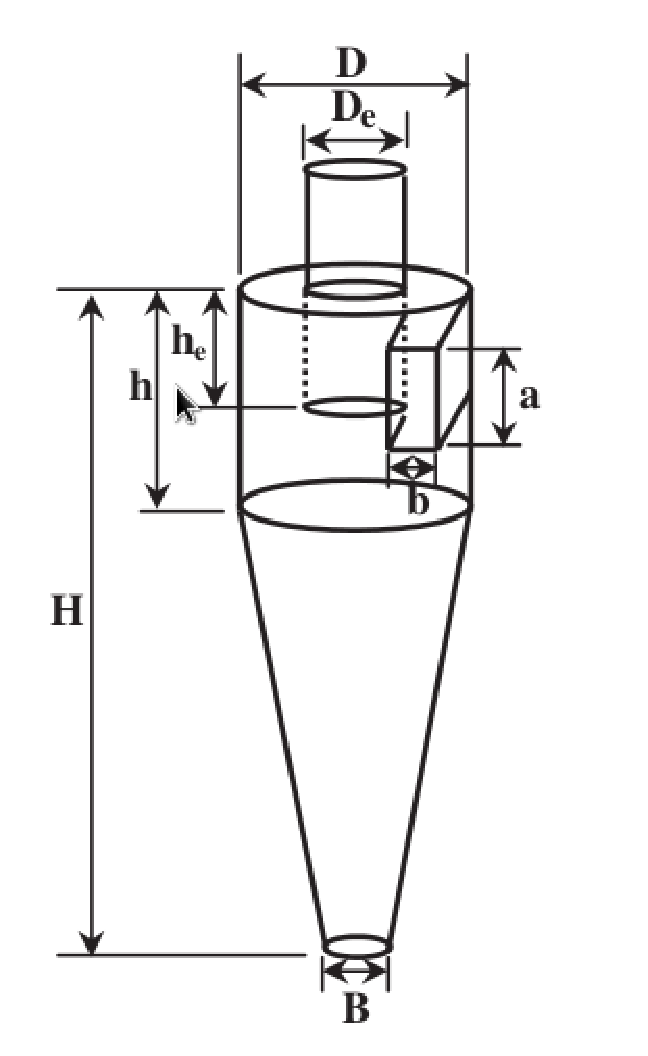
\includegraphics[scale=0.375]{Geometry}
				\captionof{figure}{Схема фильтра}
  \end{minipage}
%Решение
\newpage
\begin{thebibliography}{9}
\bibitem{Monson} Monson, D. J., Seegmiller, H. L., Mc Connaughey, P. K., and Chen, Y. S., “Comparison of Experiment With Calculations Using Curvature-Corrected Zero and Two Equation Turbulence Models for a Two-Dimensional U-Duct”, AIAA Paper No. 90-1484, 1990
\bibitem{DirgoLeith} Dirgo, J., and Leith, D., “Cyclone collection efficiency: comparison of experimental results with theoretical predictions”, Aerosol Sci. Tech. 4 410–415, 1985
\bibitem{instructions} Ужов, В.Н, “Циклоны НИИОГАЗ. Руководящие указания по проектированию, изготовлению, монтажу и эксплуатации Ярославль”, 1970
\bibitem{Menter} Menter, F., and Esch, T. “Elements of Industrial Heat Transfer Prediction”, 16th Brazilian Congress of Mechanical Engineering (COBEM), Nov. 2001
\bibitem{Garbarek} Гарбарук, А.В., “Конспект лекций дисциплины «Течения вязкой жидкости и модели турбулентности: методы расчета турбулентных течений»”, 2010
\bibitem{ShurSpallart}  Spalart, P. R., and Shur, M. L., “On the Sensitization of Turbulence Models to Rotation and Curvature”, Aerosp. Sci. Technol., 15, 1997
\bibitem{Smirnov} Smirnov, P.E., and Menter, F. R., “Sensitization of the SST Turbulence Model to Rotation and Curvature by Applying the Spalart–Shur Correction Term”, Journ. of Turbom., Volume 131, No. 4, 2009
\bibitem{CC2} Wilcox, D. C., and Chambers, T. L., “Sreamline Curvature Effects on Turbulent Boundary Layers”, AZAA J., 1977, Vol. 15, No. 4, 574-580.
\bibitem{CC3} Lien, F. S., and Leschziner, M. A., “Modeling 2D Separation From a High Lift Aerofoil with a Non-Linear Eddy-Viscosity Model and Second-Moment Closure”, Aeronautical J., April 1995. 125-144
%\bibitem{Knight} Knight, D. D., and Saffman, P. G., “Turbulence Model Predictions for Flows with Significant Mean Stramline Curvature”, AZAA-78-258
\bibitem{Bradshaw} Bradshaw, P., “Effects of Streamline Curvature on Turbulent Flow”, AGARD-AG-169, 1973
\bibitem{Speziale} Speziale, C. G., “Analytical Methods for the Development of Reynolds-Stress Closures in Turbulence”, Ann. Rev. Fluid Mech. Vol. 23, 1991, 107-157
\bibitem{Govindaraju} Govindaraju, S. P., Saffman, P. G., “Flow in a Turbulent Trailing Vortex”, Phys. Fluids, 1971
\bibitem{OPNFPG} OpenFOAM Programmer’s Guide, 2011
\bibitem{openfoam} Официальный сайт OpenFOAM, \url{http://www.openfoam.com}
\bibitem{emissionInfoRussian} Загрязнение окружающей среды в субъектах РФ, \url{http://protown.ru/information/hide/2659.html}
\bibitem{emissionInfoEurope} Wilson, A., “Cement and Concrete: Environmental Considerations”, EBN Volume 2, No. 2, 1993
\end{thebibliography}
\end{document}
